\documentclass[a4paper,12pt,twoside]{book}

% set the paper size and the margins
\usepackage[top = 2cm, bottom = 2cm, left = 2cm, right = 4cm ]{geometry}
\usepackage[showboxes]{textpos}
\setlength{\TPHorizModule}{10mm}
\setlength{\TPVertModule}{\TPHorizModule}
\TPMargin{2mm}
% set the header and the footnote
\usepackage{fancyhdr}
% Supress the hyphenation
\hyphenation{thatshouldnot}
% for table and equations
\usepackage{tablefootnote}
\usepackage{amsmath,amsfonts,amsthm}
\usepackage{multirow}
\usepackage{hhline}
% make a wide hat for the least-squares regression line
 \usepackage{scalerel,stackengine}
\stackMath
\newcommand\reallywidehat[1]{%
\savestack{\tmpbox}{\stretchto{%
  \scaleto{%
    \scalerel*[\widthof{\ensuremath{#1}}]{\kern-.6pt\bigwedge\kern-.6pt}%
    {\rule[-\textheight/2]{1ex}{\textheight}}%WIDTH-LIMITED BIG WEDGE
  }{\textheight}% 
}{0.5ex}}%
\stackon[1pt]{#1}{\tmpbox}%
}
\usepackage[shortlabels]{enumitem}

% define a color for highlight
\usepackage{xcolor}
\definecolor{asparagus}{rgb}{0.53, 0.66, 0.42}
\definecolor{babypink}{rgb}{0.96, 0.76, 0.76}
\definecolor{champagne}{rgb}{0.97, 0.91, 0.81}
\definecolor{forestgreen}{rgb}{0.13, 0.55, 0.13}
\definecolor{dollarbill}{rgb}{0.52, 0.73, 0.4}

\usepackage{tcolorbox}

\tcbset{width=0.9\textwidth,boxrule=0pt,colback=champagne,arc=0pt,
auto outer arc,left=0pt,right=0p}

\usepackage{multicol}
\usepackage{textcomp}
\usepackage{siunitx}
\usepackage{float}

\begin{document}

%Deal with the headers of each chapter
\pagestyle{fancy}
\fancyhf{}
\renewcommand{\chaptermark}[1]{ \markboth{#1}{} }
\fancyhead[CE,CO]{\leftmark}
\fancyfoot[LE,RO]{\thepage}

\chapter{One-variable data analysis}
\newpage

\begin{itemize}
\item \textbf{\large{Multiple choice}}\vspace{0.3cm}

\textbf{Section 1, Section 2, Section 3}
 \begin{enumerate}
  \item The histogram below shows the heights of 300 randomly selected high school students. Which of the following is the best description of the shape of the distribution of heights?
      \begin{figure}[H]
        \centering
         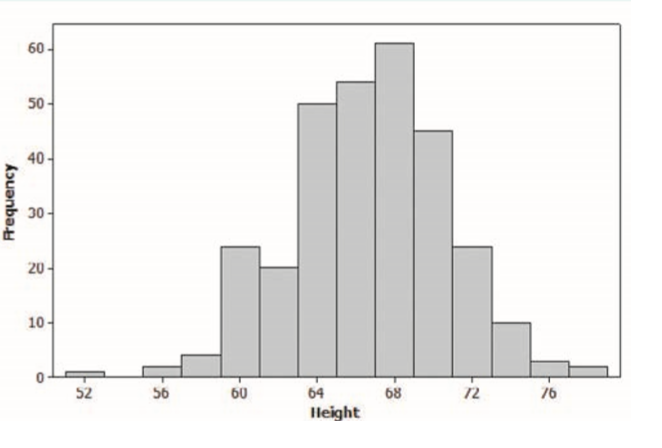
\includegraphics[scale=0.6]{figure1.png}
      \end{figure}
  
      \begin{enumerate}[(a), start = 1]
       \item Roughly symmetric and unimodal
       \item Roughly symmetric and bimodal
       \item Skewed to the left
       \item Skewed to the right
      \end{enumerate}
  \vspace{0.3cm}   
  \item You look at real estate ads for houses in Naples, Florida. There are many houses ranging from \$200,000 to \$500,000 in price. The few houses on the water, however, have prices up to \$15 million. The distribution of house prices will be 
  
    \begin{enumerate}[(a), start = 1]
    \item skewed to the left
    \item roughly symmetric
    \item skewed to the right
    \item of two clusters
    \end{enumerate}
    
 \vspace{0.3cm}
 \item  The following histogram shows the distribution of the percents of women aged 15 and over who have never married in each of the 50 states and the District of Columbia. Which of the following statements about the histogram is correct? 
 
     \begin{figure}[H]
       \centering
       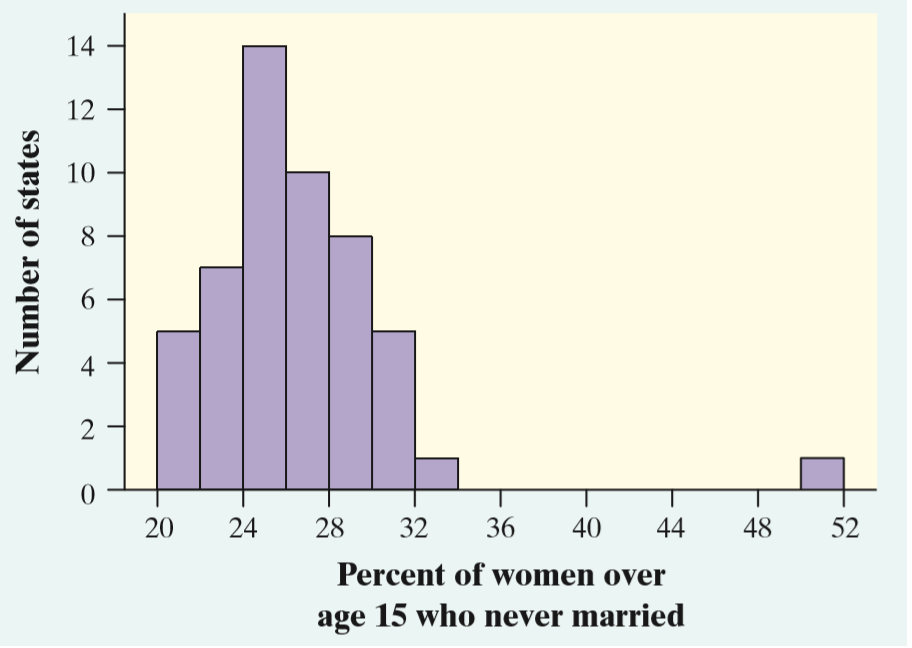
\includegraphics[scale=0.3]{figure2.png}
     \end{figure}
     
     \begin{enumerate}[(a), start = 1]
    \item The center of the distribution is about $36\%$.
    \item There are more states with percents above 32 than there are states with percents less than 24.
    \item It would be better if the values from 34 to 50 were deleted on the horizontal axis so there wouldn’t be a large gap. 
    \item There was one state with a value of exactly $33\%$.
    \item About half of the states had percents between $24\%$ and $28\%$. 
    \end{enumerate}  
    \vspace{0.3cm}  
    
 \item When comparing two distributions, it would be best to use relative frequency histograms rather than frequency histograms when 
   \begin{enumerate}[(a), start =1]
   \item the distributions have different shapes.
   \item the distributions have different spreads.
   \item the distributions have different centers.
   \item the distributions have different numbers of observations.
   \item at least one of the distributions have outliers.   
   \end{enumerate}
   \vspace{0.3cm}
   
  \item Which of the following is the best reason for choosing a stemplot rather than a histogram to display the distribution of a quantitative variable?
  
    \begin{enumerate}[(a), start = 1]
      \item Stemplots allow you to split stems; histograms don’t.
      \item Stemplots allow you to see the values of individual  observations
      \item Stemplots are better for displaying very large sets of data.
      \item Stemplots never require rounding of values.
      \item Stemplots make it easier to determine the shape of a distribution.
    \end{enumerate}
    \vspace{0.3cm}
     
   \item The scores on a statistics test had a mean of 81 and a standard deviation of 9. One student was absent on the test day, and his score wasn’t included in the calculation. If his score of 84 was added to the distribution of scores, what would happen to the mean and standard deviation?
   
     \begin{enumerate}[(a), start = 1]
       \item Mean will increase, and standard deviation will increase.
       \item Mean will increase, and standard deviation will decrease.
       \item Mean will increase, and standard deviation will stay the same.
       \item Mean will decrease, and standard deviation will increase.
       \item Mean will decrease, and standard deviation will decrease.
     \end{enumerate}
     \vspace{0.3cm}
     
   \item The stemplot shows the number of home runs hit by each of the 30 Major League Baseball teams in 2011. Home run totals above what value should be considered outliers?
   
   \begin{figure}[H]
     \centering
     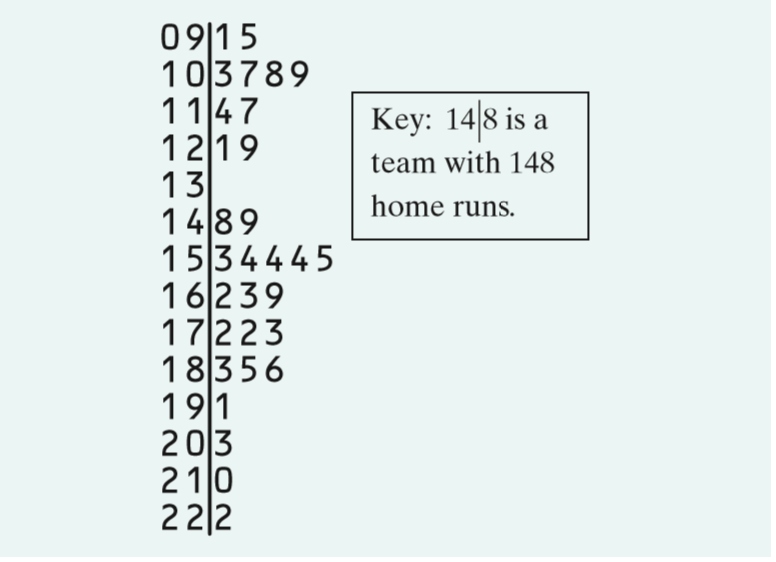
\includegraphics[scale=0.6]{figure3.png}
   \end{figure}
     
  \begin{enumerate}[(a), start = 1]
  \item 173 \hspace{0.6cm} (b) 210 \hspace{0.6cm} (c) 222, \hspace{0.6cm} (d) 229  \hspace{0.6cm} (e) 257
  \end{enumerate}
     \vspace{0.3cm}
     
     \item Which of the following boxplots best matches the distribution shown in the histogram? 
     
     \begin{figure}[H]
     \centering
     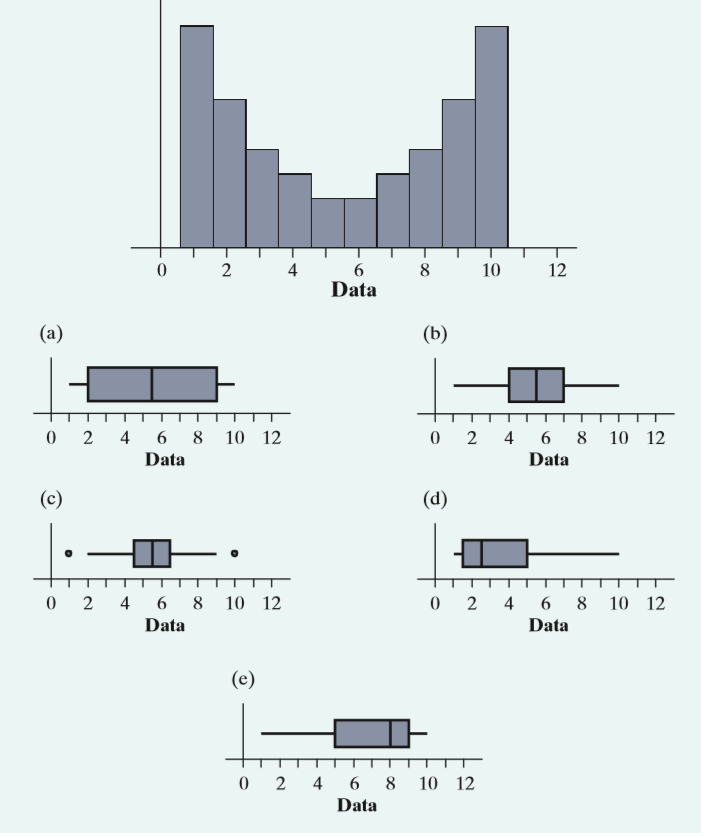
\includegraphics[scale=0.6]{figure4.png}
     \end{figure}
     
   \item You record the age, marital status, and earned income of a sample of 1463 women. The number and type of variables you have recorded is
   
   \begin{enumerate}[(a)]
     \item 3 quantitative, 0 categorical.
     \item 4 quantitative, 0 categorical.
     \item 3 quantitative, 1 categorical.
     \item 2 quantitative, 1 categorical.
     \item 2 quantitative, 2 categorical.
   \end{enumerate}
   \vspace{0.3cm}
   
   \item  In a statistics class with 136 students, the professor records how much money (in dollars) each student has in his or her possession during the first class of the semester. The histogram shows the data that were collected.
   \begin{figure}[H]
   \centering
   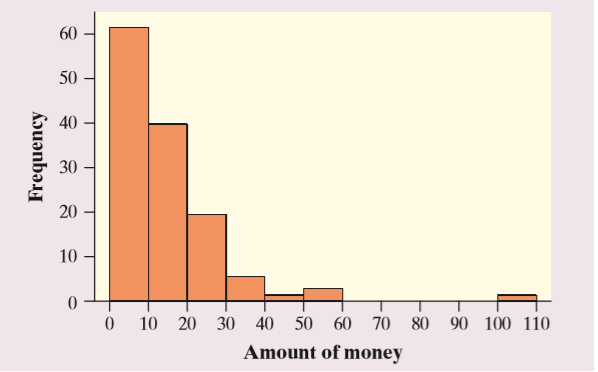
\includegraphics[scale=0.6]{figure5}
   \end{figure}

 Which of the following statements about this distribution is not correct? 
 
 \begin{enumerate}[(a), start = 1]
   \item The histogram is right-skewed.
   \item The median is less than \$20.
   \item The IQR is \$35.
   \item The mean is greater than the median.
   \item The histogram is unimodal.
 \end{enumerate}
 \vspace{0.3cm}
 
 \item An experiment was conducted to investigate the effect of a new weed killer to prevent weed growth in onion crops. Two chemicals were used: the standard weed killer (C) and the new chemical (W). Both chemicals were tested at high and low concentrations on a total of 50 test plots. The percent of weeds that grew in each plot was recorded. Here are some boxplots of the results. Which of the following is not a correct statement about the results of this experiment
 
 \begin{figure}[H]
   \centering
   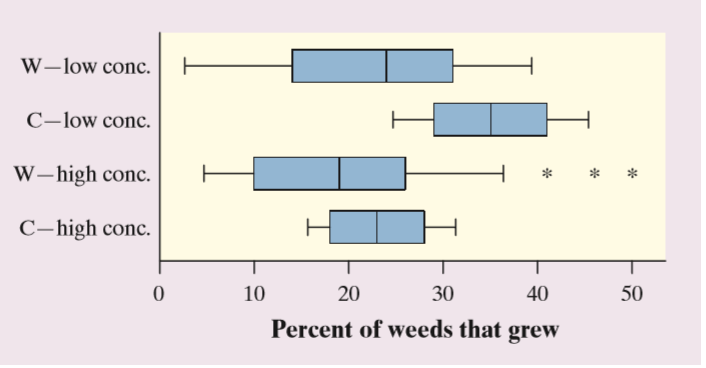
\includegraphics[scale=0.6]{figure6}
 \end{figure}
  \begin{enumerate}[(a)]
    \item At both high and low concentrations, the new chemical (W) gives better weed control than the standard weed killer (C).
    \item Fewer weeds grew at higher concentrations of both chemicals.
    \item The results for the standard weed killer (C) are less variable than those for the new chemical (W).
    \item High and low concentrations of either chemical have approximately the same effects on weed growth.
    \item Some of the results for the low concentration of weed killer W show fewer weeds growing than some of the results for the high concentration of W.
 \end{enumerate}
 \vspace{0.3cm}
 
 \item  The graph below shows household income in Laguna Woods, California.
 
    \begin{figure}[H]
      \centering
      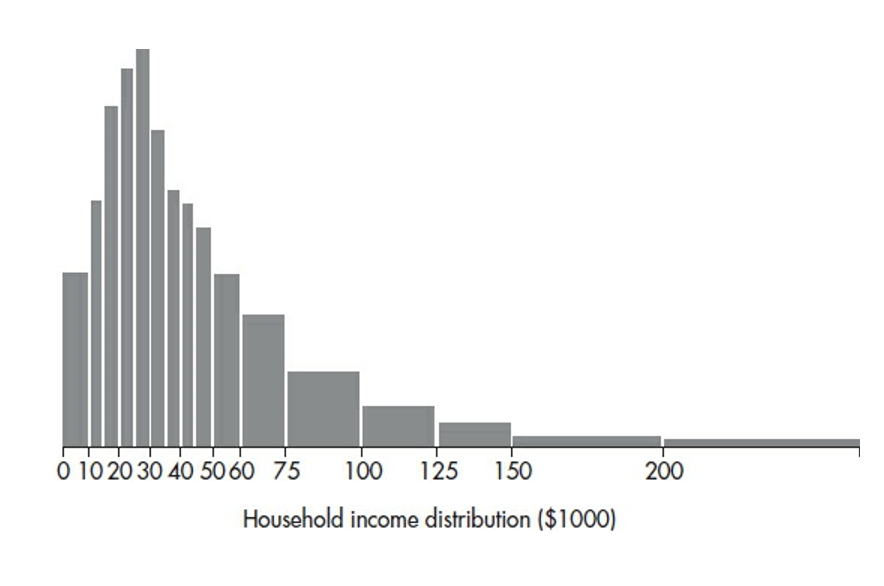
\includegraphics[scale=0.5]{figure7}
    \end{figure}

 What can be said about the ratio $\frac{\textbf{Mean family income}}{\textbf{Median family income}}$?
 
   \begin{enumerate}
     \item Approximately zero
     \item Less than one but definitely above zero
     \item Approximately one
     \item Greater than one
     \item Cannot be answered without knowing the standard deviation
   \end{enumerate}
 \vspace{0.3cm}
 
 \item Which of the following are true statements?
    \begin{enumerate}[\Roman*., start = 1]
      \item The range of the sample data set is never greater than the range of the population.
      \item The interquartile range is half the distance between the first quartile and the third quartile.
      \item  While the range is affected by outliers, the interquartile range is not. 
    \end{enumerate}
 \begin{enumerate}[(a), start = 1]
   \item I only
   \item II only
   \item III only
   \item I and II
   \item I and III
 \end{enumerate}
 \vspace{0.3cm}
 
 \item  Dieticians are concerned about sugar consumption in teenagers’ diets (a 12-ounce can of soft drink typically has 10 teaspoons of sugar). In a random sample of 55 students, the number of teaspoons of sugar consumed for each student on a randomly selected day is tabulated. Summary statistics are noted below:
 
   \begin{table}[H]
     \centering
     \begin{tabular}{cccc}
     Min = 10 & Max = 60 & $Q_1 = 25$ &  Median =31\\
     $Q_3 = 38$ & Mean = 31.4 & n = 55 & s = 11.6\\
     \end{tabular}
   \end{table}
 Which of the follwing is a true statement?
   
    \begin{enumerate}[(a), start = 1]
      \item None of the values are outliers.
      \item The value 10 is an outlier, and there can be no others.
      \item The value 60 is an outlier, and there can be no others.
      \item Both 10 and 60 are outliers, and there may be others.
      \item The value 60 is an outlier, and there may be others at the high end of the data set.
    \end{enumerate}
 
    \begin{figure}[H]
    \centering
    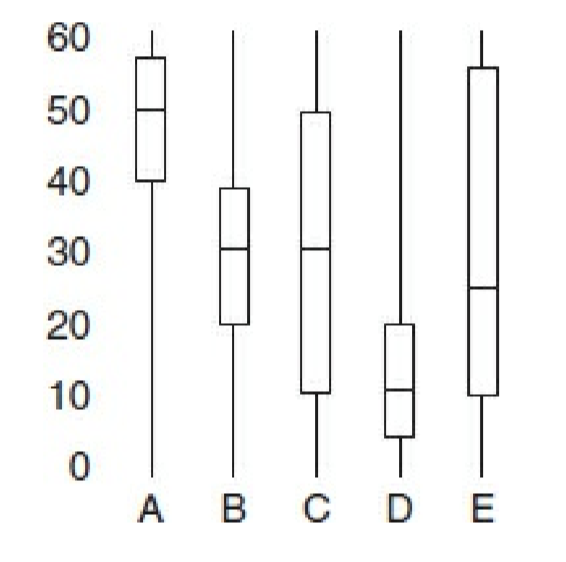
\includegraphics[scale=0.5]{figure8}
    \end{figure}
    
   \item To which of the above boxplots does the following histogram correspond?
   
     \begin{figure}[H]
     \centering
     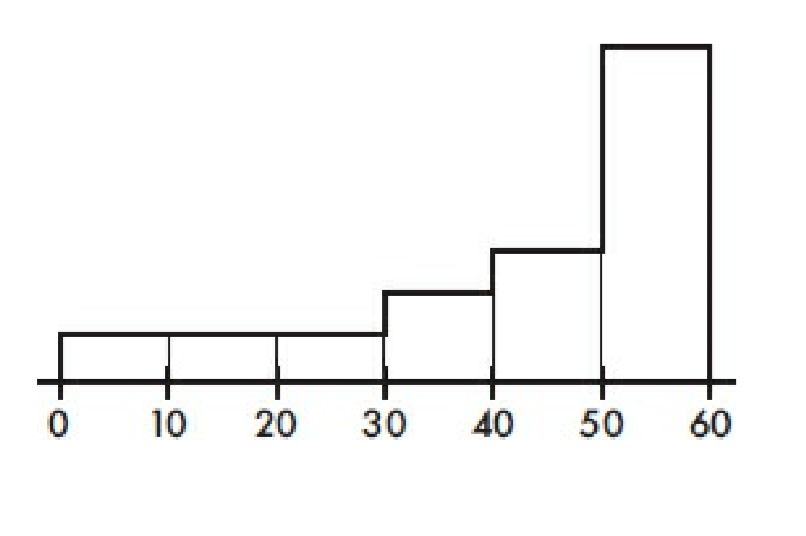
\includegraphics[scale=0.5]{figure9}
     \end{figure}
   
      \begin{enumerate}[(a)]
        \item A \hspace{0.6cm} (b) B  \hspace{0.6cm} (c) C
        \hspace{0.6cm} (d) D   \hspace{0.6cm} (e) E
      \end{enumerate}
      \vspace{0.3cm}
      
      \item Below is a boxplot of yearly tuition and fees of all four year colleges and universities in a Western state. The low outlier is from a private university that gives full scholarships to all accepted students, while the high outlier is from a private college catering to the very rich.
      \begin{figure}[H]
      \centering
       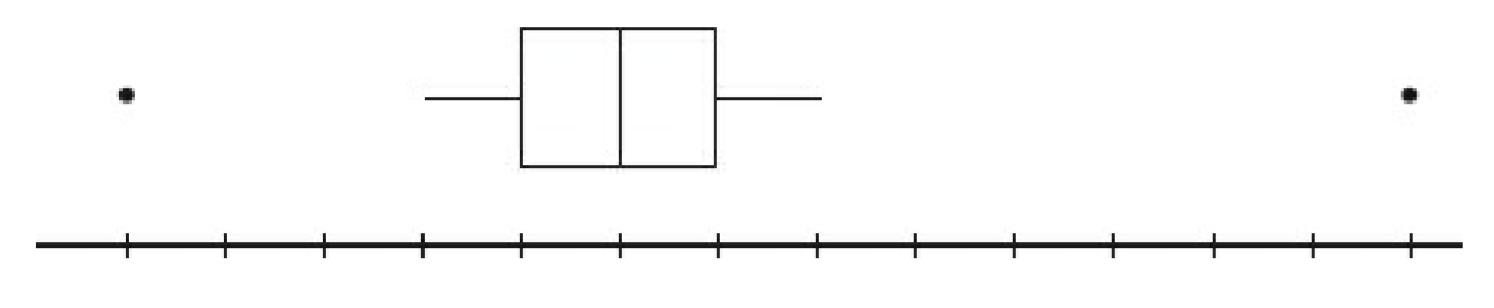
\includegraphics[scale=0.3]{figure10}
      \end{figure}
      Removing both outliers will effect what changes, if any, on the mean and median costs for this state’s four year institutions of higher learning?
      \begin{enumerate}[(a)]
        \item Both the mean and the median will be unchanged.
        \item The median will be unchanged, but the mean will increase.
        \item The median will be unchanged, but the mean will decrease.
        \item The mean will be unchanged, but the median will increase.
        \item Both the mean and median will change.
      \end{enumerate}
      \vspace{0.3cm}
   
   \item If quartiles $Q_1 = 20$ and $Q_3 = 30$, which of the following must be true?   
     \begin{enumerate}[\Roman*. , start =1]
     \item The median is 25.
     \item The mean is between 20 and 30.
     \item The standard deviation is at most 10.     
     \end{enumerate}
     
     \begin{enumerate}[(a)]
       \item I only.
       \item II only.
       \item III only.
       \item All are true.
       \item None are true.
     \end{enumerate}
      \vspace{0.3cm}
      
     \item A 1995 poll by the Program for International Policy asked respondents what percentage of the U.S. budget they thought went to foreign aid. The mean response was 18\%, and the median was 15\%. (The actual amount is less than 1\%.) What do these responses indicate about the likely shape of the distribution of all the responses?
     
     \begin{enumerate}[(a)]
       \item The distribution is skewed to the left.
       \item The distribution is skewed to the right.
       \item The distribution is symmetric around 16.5\%.
       \item  The distribution is bell-shaped with a standard deviation of 3\%.
       \item The distribution is uniform between 15\% and 18\%.
     \end{enumerate}
     \vspace{0.3cm}
     
    \item Which of the following are true statements?
      \begin{enumerate}[\Roman*. , start =1]
        \item If the sample has variance zero, the variance of the population is also zero.
        \item If the population has variance zero, the variance of the sample is also zero.
        \item If the sample has variance zero, the sample mean and the sample median are equal.
      \end{enumerate}
      
        \begin{enumerate}[(a)]
           \item I and II
           \item II and III
           \item I and III
           \item I, II and III
           \item None of the above
        \end{enumerate}
        \vspace{0.3cm}
        
        \item When a set of data has suspect outliers, which of the following are preferred measures of central tendency and of variability?
        \begin{enumerate}[(a)]
          \item mean and standard deviation
          \item mean and variance
          \item mean and range
          \item median and range
          \item median and interquartile range
        \end{enumerate}
        \vspace{0.3cm}
        
    \item The 70 highest dams in the world have an average height of 206 meters with a standard deviation of 35 meters. The Hoover and Grand Coulee dams have heights of 221 and 168 meters, respectively. The Russian dams, the Nurek and Charvak, have heights with z-scores of +2.69 and – 1.13, respectively. List the dams in order of ascending size.
    \begin{enumerate}[(a)]
      \item Charvak, Grand Coulee, Hoover, Nurek
      \item Charvak, Grand Coulee, Nurek, Hoover
      \item Grand Coulee, Charvak, Hoover, Nurek
      \item Grand Coulee, Charvak, Nurek, Hoover
      \item Grand Coulee, Hoover, Charvak, Nurek
    \end{enumerate}
    \vspace{0.3cm}
    
    \item Jorge’s score on Exam 1 in his statistics class was at the 64th percentile of the scores for all students. His score falls
    
    \begin{enumerate}[(a)]
        \item between the minimum and the first quartile.
        \item between the first quartile and the median.
        \item between the median and the third quartile.
        \item between the third quartile and the maximum.
        \item at the mean score for all students.
    \end{enumerate}
    \vspace{0.3cm}
    
    \item When Sam goes to a restaurant, he always tips the server \$2 plus 10\% of the cost of the meal. If Sam’s distribution of meal costs has a mean of \$9 and a standard deviation of \$3, what are the mean and standard deviation of the distribution of his tips?
    
        \begin{enumerate}[(a)]
            \item  \$2.90, \$0.30
            \item  \$2.90, \$2.30
            \item  \$9.00, \$3.00
            \item  \$11.00, \$2.00
            \item  \$2.00, \$9.00
        \end{enumerate}
        \vspace{0.3cm}
        
    \item George has an average bowling score of 180 and bowls in a league where the average for all bowlers is 150 and the standard deviation is 20. Bill has an average bowling score of 190 and bowls in a league where the average is 160 and the standard deviation is 15. Who ranks higher in his own league, George or Bill?
        
        \begin{enumerate}[(a)]
            \item Bill, because his 190 is higher than George’s 180.
            \item Bill, because his standardized score is higher than George’s.
            \item Bill and George have the same rank in their leagues, because both are 30 pins above the mean.
            \item George, because his standardized score is higher than Bill’s.
            \item George, because the standard deviation of bowling scores is higher in his league.
        \end{enumerate}
        \vspace{0.3cm}
        
    \textit{The following two problems refer to the following setting.} The number of absences during the fall semester was recorded for each student in a large elementary school. The distribution of absences is displayed in the following cumulative relative frequency graph.
    \begin{figure}[H]
        \centering
        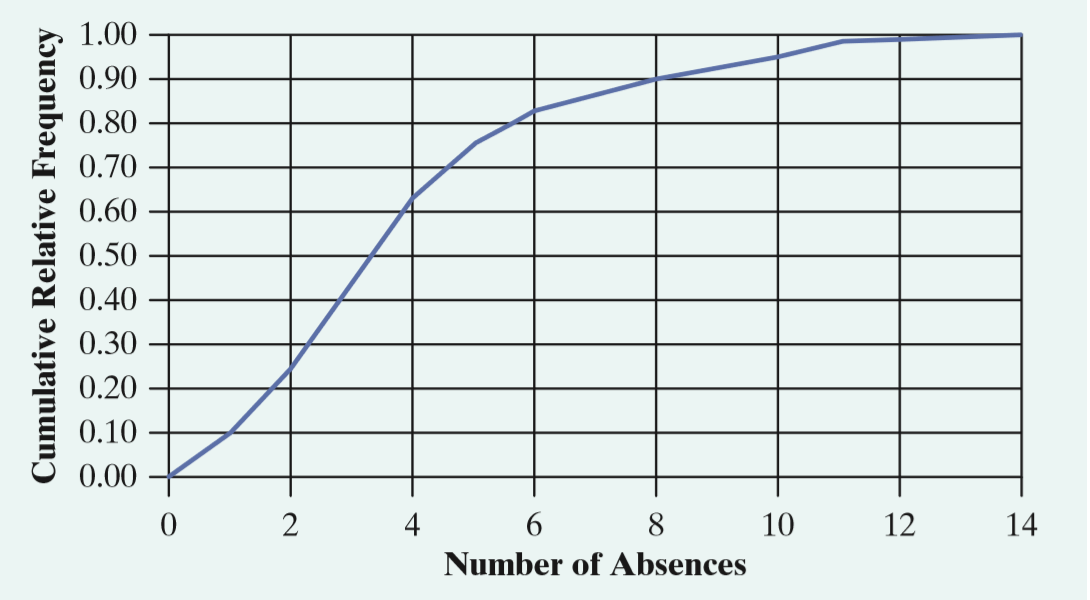
\includegraphics[scale=0.4]{figure11}
    \end{figure}

    \item What is the interquartile range (IQR) for the distribution of absences?
    
        \begin{enumerate}[(a)]
            \item 1 \hspace{0.6cm} (b) 2 \hspace{0.6cm} (c) 3
            \hspace{0.6cm} (d) 5    \hspace{0.6cm} (e) 14
        \end{enumerate}
        
   \item If the distribution of absences was displayed in a histogram, what would be the best description of the histogram’s shape?
   
       \begin{enumerate}[(a)]
       \item Symmetric
       \item Uniform
       \item left-skewed
       \item right-skewed
       \item can not be determined
       \end{enumerate}  
       
       
   \item Two measures of center are marked on the density curve shown. Which of the following is correct?
       \begin{figure}[H]
       \centering
       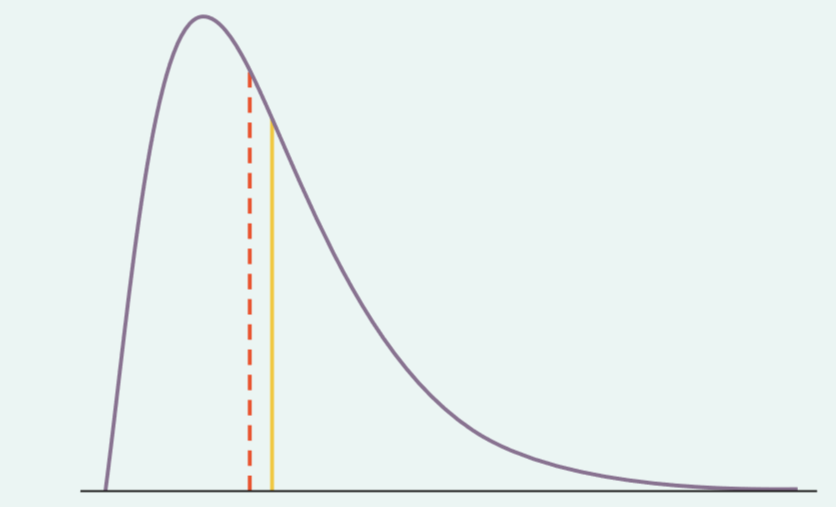
\includegraphics[scale=0.5]{figure12}
       \end{figure}    
       
       \begin{enumerate}[(a)]
           \item The median is at the solid line and the mean is at the dashed line.
           \item The median is at the dashed line and the mean is at the solid line.
           \item The mode is at the dashed line and the median is at the solid line.
           \item The mode is at the solid line and the median is at the dashed line.
           \item  The mode is at the dashed line and the mean is at the solid line.
       \end{enumerate}   
        
   \item   Many professional schools require applicants to take a standardized test. Suppose that 1000 students take such a test. Several weeks after the test, Pete receives his score report: he got a 63, which placed him at the 73rd percentile. This means that 
   
       \begin{enumerate}[(a)]
           \item Pete’s score was below the median.
           \item Pete did worse than $63\%$ of the test takers.
           \item Pete did worse than $73\%$ of the test takers.
           \item Pete did better than $63\%$ of the test takers.
           \item Pete did better than $73\%$ of the test takers.
       \end{enumerate}        
         \vspace{0.3cm}
   
   \item  For the Normal distribution shown, the standard deviation is closest to
       \begin{figure}[H]
           \centering
           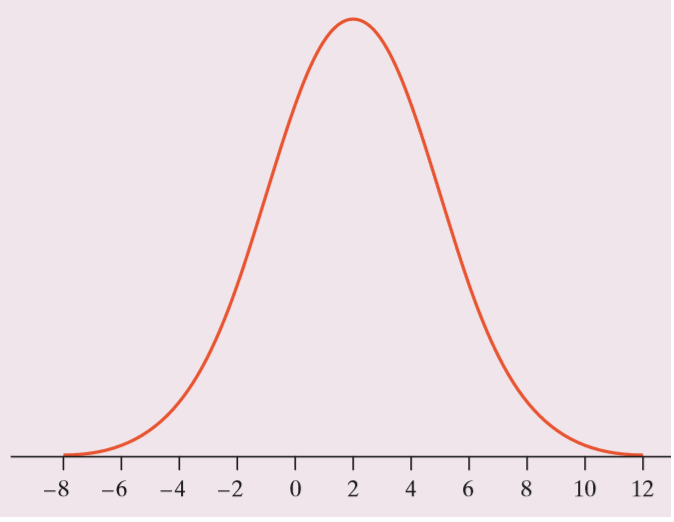
\includegraphics[scale=0.5]{figure13}
       \end{figure}
       
       \begin{multicols}{5}
       \begin{enumerate}[(a), start = 1]
           \item 0
           \item 1
           \item 2
           \item 3
           \item 5
       \end{enumerate}
       \end{multicols}
       
   \item The figure shows a cumulative relative frequency graph of the number of ounces of alcohol consumed per week in a sample of 150 adults who report drinking alcohol occasionally. About what percent of these adults consume between 4 and 8 ounces per week?
   
     \begin{figure}[H]
         \centering
         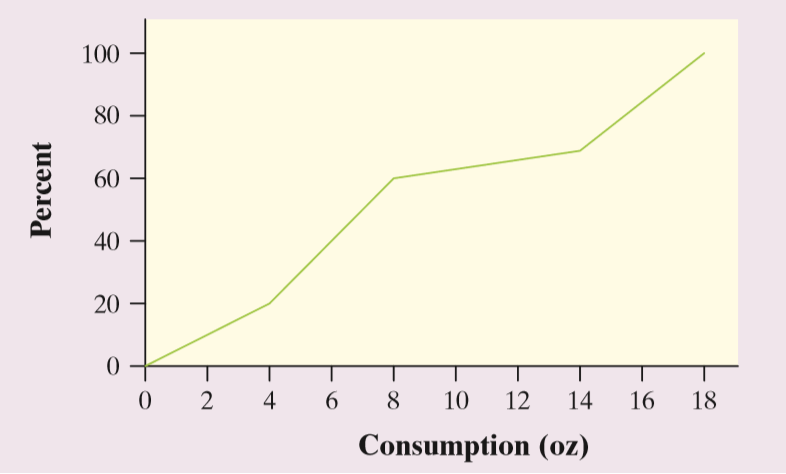
\includegraphics[scale=0.5]{figure14}
     \end{figure}
     
     \begin{multicols}{5}
         \begin{enumerate}[(a)]
             \item $20\%$
             \item $40\%$
             \item $50\%$
             \item $60\%$
             \item $80\%$
         \end{enumerate}
     \end{multicols}
     
  \item Which of the following is not correct about a standard Normal distribution
   
   \begin{enumerate}[(a)]
       \item  The proportion of scores that satisfy $0 < z < 1.5$ is 0.4332.
       \item The proportion of scores that satisfy $z < −1.0$ is 0.1587.
       \item  The proportion of scores that satisfy $z > 2.0$ is 0.0228.
       \item The proportion of scores that satisfy $z < 1.5$ is 0.9332.
       \item The proportion of scores that satisfy $z > −3.0$ is 0.9938.
   \end{enumerate}
   \vspace{0.3cm}  
   
  \textit{The next two problems refer to the following setting.}  Until the scale was changed in 1995, SAT scores were based on a scale set many years ago. For Math scores, the mean under the old scale in the 1990s was 470 and the standard deviation was 110. In 2009, the mean was 515 and the standard deviation was 116.
  
  \item  What is the standardized score (z-score) for a student who scored 500 on the old SAT scale?
  \begin{multicols}{5}
  \begin{enumerate}[(a)]
      \item -30
      \item -0.27
      \item -0.13
      \item 0.13
      \item 0.27
  \end{enumerate}
  \end{multicols}
   
 \item  Gina took the SAT in 1994 and scored 500. Her cousin Colleen took the SAT in 2013 and scored 530. Who did better on the exam, and how can you tell?
    \begin{enumerate}[(a)]
        \item  Colleen, she scored 30 points higher than Gina
        \item  Colleen, her standardized score is higher than Gina’s.
        \item Gina, her standardized score is higher than Colleen’s.
        \item Gina, the standard deviation was bigger in 2013.
        \item The two cousins did equally well—their z-scores are the same.
    \end{enumerate}      
   \vspace{0.3cm}
   
    \item Which of the following can be used to describe the center of a data set?
      \begin{enumerate}[(a)]
          \item $\frac{Q_1-Q_3}{2}$
          \item $\frac{Q_1+Q_3}{2}$
          \item $\frac{\text{range}}{2}$
          \item $\frac{\text{Standard deviation}}{2}$
      \end{enumerate}
      \vspace{0.3cm}
      
  \item A set of 5,000 scores on a college readiness exam are known to be approximately normally distributed with mean 72 and standard deviation 6. To the nearest integer value, how many scores are there between 63 and 75?
      \begin{enumerate}[(a)]
          \item 0.6247
          \item 4,115
          \item 3,650
          \item 3,123
          \item 3,227
      \end{enumerate}
      \vspace{0.3cm}
       
    \item Free-response questions on the AP Statistics Exam are graded on 4, 3, 2, 1 or 0 basis. Question \# 2 on the exam was of moderate difficulty. The average score on question \# 2 was 2.05, with a standard deviation of 1. To the nearest tenth, what score was achieved by a student who was at the 90th percentile of all students on the test? You may assume that the scores on the question were approximately normally distributed.
    
        \begin{enumerate}[(a)]
            \item 3.5
            \item 3.3
            \item 2.9
            \item 3.7
            \item 3.1
        \end{enumerate}                 
 \end{enumerate}
 \newpage
 
 \item {\large{\textbf{Free Response}}}
 
 \begin{enumerate}
     \item \textbf{Do pets or friends help reduce stress}
     
     If you are a dog lover, having your dog with you may reduce your stress level. Does having a friend with you reduce stress? To examine the effect of pets and friends in stressful situations, researchers recruited 45 women who said they were dog lovers. Fifteen women were assigned at random to each of three groups: to do a stressful task alone, with a good friend present, or with their dogs present. The stressful task was to count backward by 13s or 17s. The woman’s average heart rate during the task was one measure of the effect of stress. The table below shows the data.
    
     \begin{minipage}{0.85\textwidth}
     \begin{figure}[H]
     \centering
     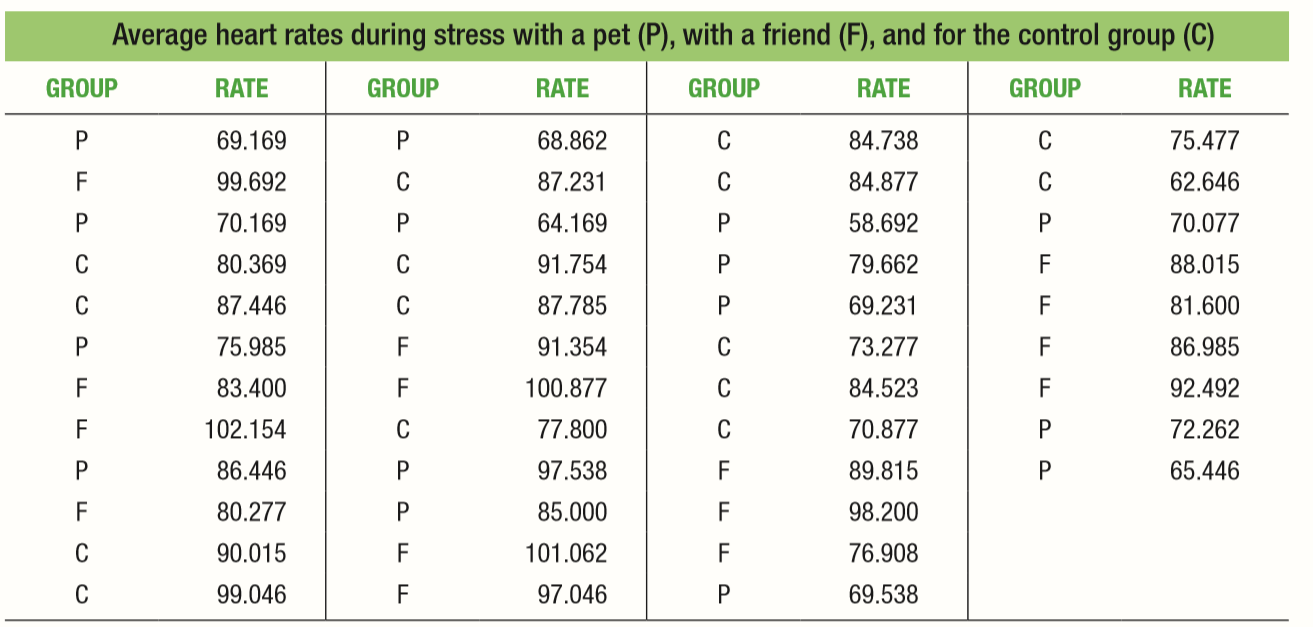
\includegraphics[scale=0.6]{figure15}
     \end{figure}
     \end{minipage}

 Use what you have learnt in this chapter to analyze the data.
     \begin{enumerate}[(a)]
         \item Construct an appropriate graph for comparing the heart rates of the women in the three groups.
         \item Calculate numerical summaries for each group’s data. Which measures of center and spread would you choose to compare? Why?
         \item Determine if there are any outliers in each of the three groups. Show your work.
         \item Write a few sentences comparing the distributions of heart rates for the women in the three groups.
         \item Based on the data, does it appear that the presence of a pet or friend reduces heart rate during a stressful task? Justify your answer.           
     \end{enumerate}
     \newpage
     
     \item \textbf{I think I can}
     
      An important measure of the performance of a locomotive is its “adhesion,” which is the locomotive’s pulling force as a multiple of its weight. The adhesion of one 4400-horsepower diesel locomotive varies in actual use according to a Normal distribution with mean $\mu = 0.37$ and standard deviation  $\sigma = 0.04$. 
      
      \begin{enumerate}[(a)]
          \item For a certain small train’s daily route, the locomotive needs to have an adhesion of at least 0.30 for the train to arrive at its destination on time. On what proportion of days will this happen? Show your method.
          \item An adhesion greater than 0.50 for the locomotive will result in a problem because the train will arrive too early at a switch point along the route. On what proportion of days will this happen? Show your method.
      \end{enumerate}
      
       The locomotive’s manufacturer is considering two changes that could reduce the percent of times that the train arrives late. One option is to increase the mean adhesion of the locomotive. The other possibility is to decrease the variability in adhesion from trip to trip, that is, to reduce the standard deviation. 
       
       \begin{enumerate}[(a), resume]
       \item  If the standard deviation remains at $\sigma = 0.04$, to what value must the manufacturer change the mean adhesion of the locomotive to reduce its proportion of late arrivals to only 2\% of days? Show your work.
       \item  If the mean adhesion stays at $\mu = 0.37$, how much must the standard deviation be decreased to ensure that the train will arrive late only 2\% of the time? Show your work.
       \item Which of the two options in parts (a) and (b) do you think is preferable? Justify your answer. (Be sure to consider the effect of these changes on the percent of days that the train arrives early to the switch point.)
       \end{enumerate}
       \newpage
 
 \item The distribution of scores on a recent test closely followed a Normal distribution with a mean of 22 points and a standard deviation of 4 points. 
 
    \begin{enumerate}[(a)]
        \item What proportion of the students scored at least 25 points on this test?
        \item What is the 31st percentile of the distribution of test scores?
        \item The teacher wants to transform the test scores so that they have an approximately Normal distribution with a mean of 80 points and a standard deviation of 10 points. To do this, she will use a formula in the form:
        $$new score = a + b (old score)$$
Find the values of a and b that the teacher should use to transform the distribution of test scores.
        \item Before the test, the teacher gave a review assignment for homework. The maximum score on the assignment was 10 points. The distribution of scores on this assignment had a mean of 9.2 points and a standard deviation of 2.1 points. Would it be appropriate to use a Normal distribution to calculate the proportion of students who scored below 7 points on this assignment? Explain.
    \end{enumerate}
    \newpage
    
    
     \item \textbf{2006FRB1}\\
    A large regional real estate company keeps records of home sales for each of its sales agents. Each month, the company publishes the sales volume for each agent. Monthly sales volume is defined as the total sales price of all homes sold by the agent during a month. The figure below displays the cumulative relative frequency plot of the most recent monthly sales volume (in hundreds of thousands of dollars) for these agents.
       \begin{center}
       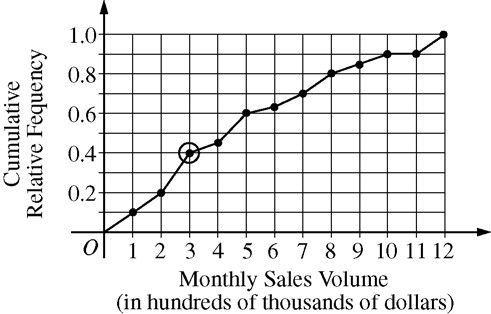
\includegraphics[scale=0.5]{2006FRB1.JPG}
       \end{center}
    \begin{enumerate}[label = (\alph*)]
      \item  In the context of this question, explain what information is conveyed by the circled point.
      \item  What proportion of sales agents achieved monthly sales volumes between \$700,000 and \$800,000?
      \item For values between 10 and 11 on the horizontal axis, the cumulative relative frequency plot is flat. In the context of this question, explain what this means.
      \item A bonus is to be given to 20 percent of the sales agents. Those who achieved the highest monthly sales volume during the preceding month will receive a bonus. What is the minimum monthly sales volume an agent must have achieved to qualify for the bonus?
      \end{enumerate}
 \end{enumerate}
\end{itemize}

\chapter{Two-variable data analysis}
\newpage

\textbf{Multiple Choice}

    \begin{enumerate}   
    \item In the 2010\textendash 2011 season, the Dallas Mavericks won the NBA championship. The two-way table below displays the relationship between the outcome of each game in the regular season and whether the Mavericks scored at least 100 points. 
        \begin{figure}[H]
            \centering
            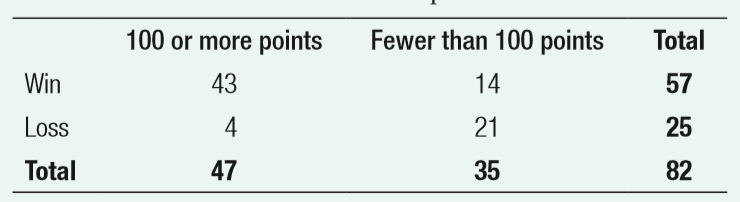
\includegraphics[scale=0.6]{figure0201}
        \end{figure}
    Which of the following is the best evidence that there is an association between the outcome of a game and whether or not the Mavericks scored at least 100 points?
    
        \begin{enumerate}[(a)]
            \item The Mavericks won 57 games and lost only 25 games.
            \item The Mavericks scored at least 100 points in 47 games and fewer than 100 points in only 35 games.
            \item The Mavericks won 43 games when scoring at least 100 points and only 14 games when scoring fewer than 100 points. 
            \item The Mavericks won a higher proportion of games when scoring at least 100 points (43/47) than when they scored fewer than 100 points (14/35).
            \item The combination of scoring 100 or more points and winning the game occurred more often (43 times) than any other combination of outcomes.
        \end{enumerate}
        \vspace{0.3cm}
        
    \item The following partially complete two-way table shows the marginal distributions of gender and handedness for a sample of 100 high school students.
    
        \begin{figure}[H]
            \centering
            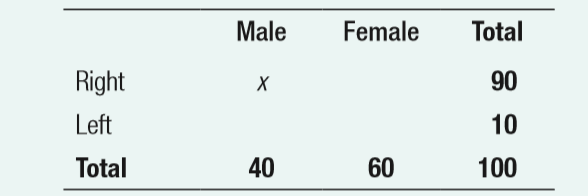
\includegraphics[scale=0.6]{figure0202}
        \end{figure}
    If there is no association between gender and handedness for the members of the sample, which of the following is the correct value of $x$?
        \begin{multicols}{4}
        \begin{enumerate}[(a)]
            \item 20
            \item 30
            \item 36
            \item 45
        \end{enumerate}
        \end{multicols}
        \begin{enumerate}[(a), resume]
            \item Impossible to determine without more information.
        \end{enumerate}
        \vspace{0.3cm}
    
    
    \item You have data for many years on the average price of a barrel of oil and the average retail price of a gallon of unleaded regular gasoline. If you want to see how well the price of oil predicts the price of gas, then which should be taken as the explanatory variable?
    
    \begin{enumerate}[(a)]
        \item the price of oil
        \item the price of gas
        \item the year
        \item either oil or gas price
        \item time
    \end{enumerate}

    
\item The following graph plots the gas mileage (miles per gallon) of various cars from the same model year versus the weight of these cars in thousands of pounds. The circles correspond to cars made in Japan. From this plot, we may conclude that
    \begin{figure}[H]
        \centering
        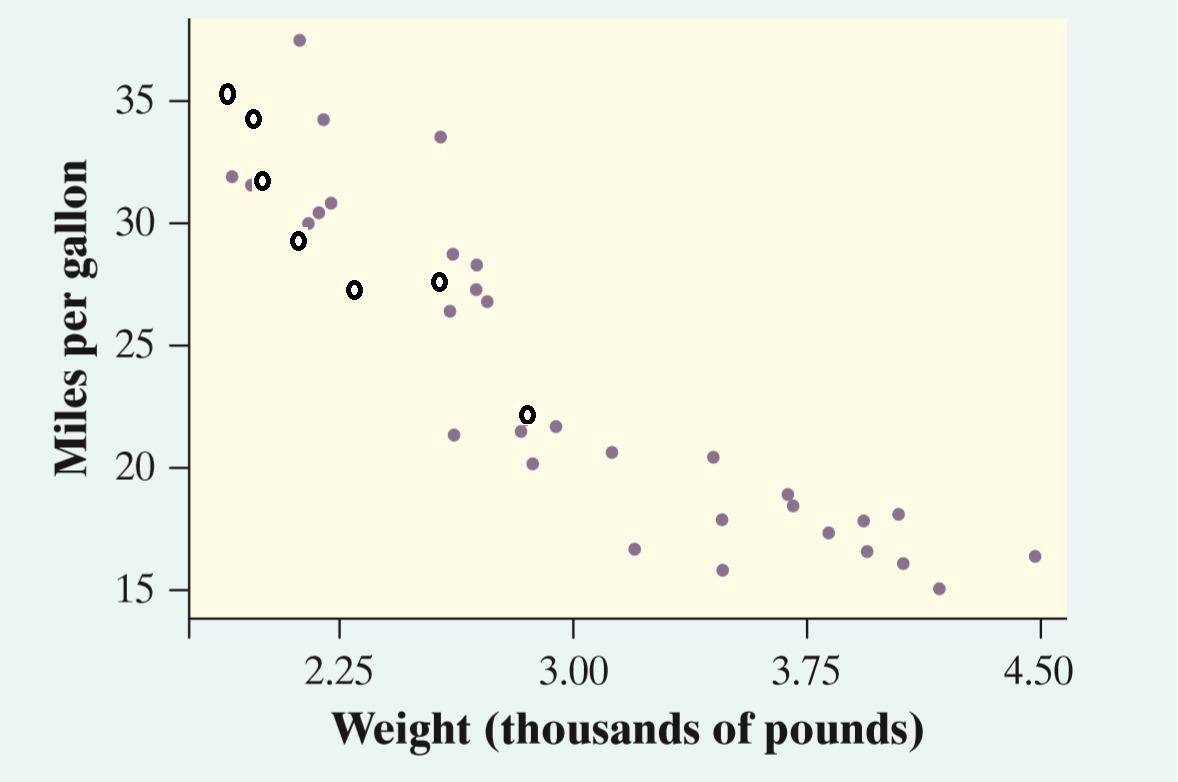
\includegraphics[scale=0.3]{figure0203}
    \end{figure}
    \begin{enumerate}[(a)]
        \item there is a positive association between weight and gas mileage for Japanese cars.
        \item the correlation between weight and gas mileage for all the cars is close to 1.
        \item there is little difference between Japanese cars and cars made in other countries.
        \item Japanese cars tend to be lighter in weight than other cars.
        \item Japanese cars tend to get worse gas mileage than other cars.
    \end{enumerate}
    \vspace{0.3cm}

\item If women always married men who were 2 years older than themselves, what would the correlation between the ages of husband and wife be?

     \begin{multicols}{4}
     \begin{enumerate}[(a)]
         \item 2
         \item 1
         \item 0.5
         \item 0
     \end{enumerate}
     \end{multicols}
     \begin{enumerate}[(e)]
         \item Can’t tell without seeing the data
     \end{enumerate}
     \vspace{0.3cm}
     
 \item The figure below is a scatterplot of reading test scores against IQ test scores for 14 fifth-grade children. There is one low outlier in the plot. What effect does this low outlier have on the correlation?
     \begin{figure}[H]
     \centering
     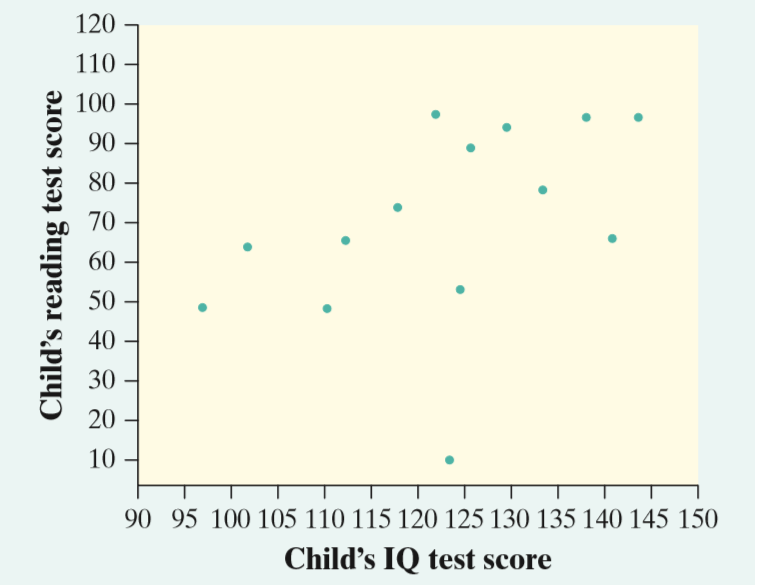
\includegraphics[scale=0.5]{figure0204}
     \end{figure}
     
     \begin{enumerate}[(a)]
         \item It makes the correlation closer to 1.
         \item It makes the correlation closer to 0 but still positive.
         \item It makes the correlation equal to 0.
         \item It makes the correlation negative.
         \item It has no effect on the correlation.
     \end{enumerate}
     \vspace{0.3cm}
     
 \item Which of the following is not a characteristic of the least-squares regression line?
     \begin{enumerate}[(a)]
         \item The slope of the least-squares regression line is always between $-1$ and $1$.
         \item The least-squares regression line always goes through the point $(\bar{x}, \bar{y})$.
         \item The least-squares regression line minimizes the sum of squared residuals.
         \item The slope of the least-squares regression line will always have the same sign as the correlation
         \item The least-squares regression line is not resistant to outliers.
     \end{enumerate}
     \vspace{0.3cm}
     
 \item  Each year, students in an elementary school take a standardized math test at the end of the school year. For a class of fourth-graders, the average score was 55.1 with a standard deviation of 12.3. In the third grade, these same students had an average score of 61.7 with a standard deviation of 14.0. The correlation between the two sets of scores is r = 0.95. Calculate the equation of the least-squares regression line for predicting a fourth-grade score from a third-grade score.
 
     \begin{enumerate}[(a)]
         \item $\hat{y} = 3.60 + 0.835 \,x$
         \item $\hat{y} = 15.69 + 0.835 \,x$
         \item $\hat{y} = 2.19 + 1.08 \,x$
         \item $\hat{y} = -11.54 + 1.08\, x$
         \item Can not be calculated without the data.
     \end{enumerate}
     \vspace{0.3cm}
     
     \item Using data from the 2009 LPGA tour, a regression analysis was performed using x = average driving distance and y = scoring average. Using the output from the regression analysis shown below, determine the equation of the least-squares regression line.
         \begin{figure}[H]
             \centering
             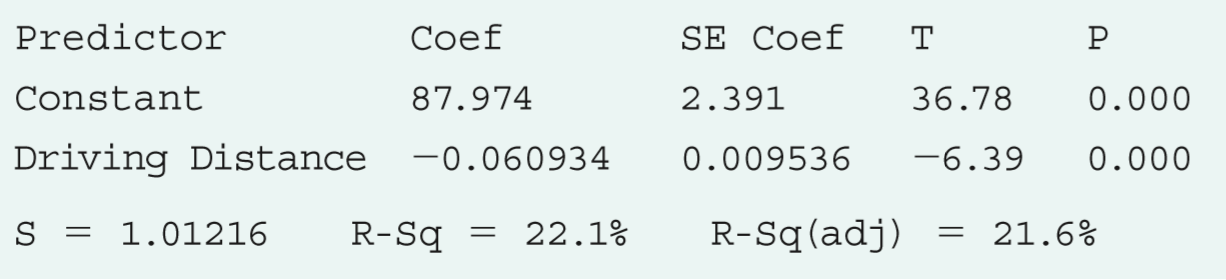
\includegraphics[scale=0.5]{figure0205}
         \end{figure}
         \begin{enumerate}[(a)]
             \item $\hat{y} = 87.947 + 2.31\,9x$
             \item $\hat{y} = 87.947 + 1.01216\,x$
             \item $\hat{y} = 87.947 - 0.060934\,x$
             \item $\hat{y} = -0.060934 + 1.01216\,x$
             \item $\hat{y} = -0.060934 + 87.947\,x$
         \end{enumerate}
         \vspace{0.3cm}
    
     \textit{The following 5 problems refer to the following setting.}
    
    Measurements on young children in Mumbai, India, found this least-squares line for predicting height y from arm span x:
    $$\hat{y} = 6.4 + 0.93\, x$$
    Measurements are in centimeters (cm).
    \vspace{0.3cm}
    
    \item By looking at the equation of the least-squares regression line, you can see that the correlation between height and arm span is
    
        \begin{enumerate}[(a)]
            \item greater than zero. 
            \item less than zero.
            \item 0.93
            \item 6.4
            \item Can not tell without seeing the data.
        \end{enumerate}
        \vspace{0.3cm}
        
    \item In addition to the regression line, the report on the Mumbai measurements says that $r^2 = 0.95$. This  suggests that
        \begin{enumerate}[(a)]
            \item although arm span and height are correlated, arm span does not predict height very accurately
            \item height increases by $\sqrt{0.95} = 0.97$ cm for each additional centimeters of arm span.
            \item 95\% of the relationship between height and arm span is accounted for by the regression line.
            \item 95\% of the variation in height is accounted for by the regression line.
            \item 95\% of the height measurements are accounted for by the regression line.
        \end{enumerate}
        \vspace{0.3cm}
        
    \item One child in the Mumbai study had height 59 cm and arm span 60 cm. This child’s residual is
    \begin{multicols}{5}
        \begin{enumerate}[(a)]
            \item $-3.2$ cm
            \item $-2.2$ cm
            \item $-1.3$ cm
            \item $3.2$ cm
            \item $62.2$ cm
        \end{enumerate}
     \end{multicols}
     \vspace{0.3cm}
     
  \item Suppose that a tall child with arm span 120 cm and height 118 cm was added to the sample used in this study. What effect will adding this child have on the correlation and the slope of the least-squares regression line?
      \begin{enumerate}[(a)]
          \item Correlation will increase, slope will increase.
          \item Correlation will increase, slope will stay the same.
          \item Correlation will increase, slope will decrease.
          \item Correlation will stay the same, slope will stay the same.
          \item Correlation will stay the same, slope will increase.
      \end{enumerate}
      \vspace{0.3cm}
    
   \item Suppose that the measurements of arm span and height were converted from centimeters to meters by dividing each measurement by 100. How will this conversion affect the values of $r^2$ and $s$?
   
       \begin{enumerate}[(a)]
           \item $r^2$  will increase, $s$ will increase.
           \item $r^2$  will increase, $s$ will stay the same.
           \item $r^2$  will increase, $s$ will decrease.
           \item $r^2$  will stay the same, $s$ stay the same.
           \item $r^2$  will stay the same, $s$ will decrease.
       \end{enumerate}
       \vspace{0.3cm}
       
   \item The fraction of the variation in the values of y that is explained by the least-squares regression of y on x is
       \begin{enumerate}[(a)]
           \item the correlation.
           \item the slope of the least-squares regression line.
           \item the square of the correlation coefficient.
           \item the intercept of the least-squares regression line.
           \item the residual.
       \end{enumerate}
       \vspace{0.3cm}
       
   \item  An AP\textsuperscript{\textregistered} Statistics student designs an experiment to see whether today’s high school students are becoming too 
 calculator-dependent. She prepares two quizzes, both of which contain 40 questions that are best done using paper-and-pencil methods. A random sample of 30 students participates in the experiment. Each student takes both quizzes \textemdash one with a calculator and one without\textemdash \,in a random order. To analyze the data, the student constructs a scatterplot that displays the number of correct answers with and without a calculator for each of the 30 students. A least-squares regression yields the equation
        $$\reallywidehat{\text{Calculator}} = -1.2+0.865\,(\text{Pencil}), \hspace{0.6cm r = 0.79}$$
    Which of the following statements is/are true?
    
        \begin{enumerate}[\Roman*. , start =1]
            \item If the student had used Calculator as the explanatory variable, the correlation would remain the same.
            \item If the student had used Calculator as the explanatory variable, the slope of the least-squares line would remain the same.
            \item The standard deviation of the number of correct answers on the paper-and-pencil quizzes was larger than the standard deviation on the calculator quizzes.
        \end{enumerate}
        
        \begin{multicols}{3}
        \begin{enumerate}[(a)]
           \item I only    \item II only    \item III only
           \item I and III only     \item I, II and III           
        \end{enumerate}
        \end{multicols}
        \vspace{0.3cm}
        
\textit{The following two problems refer to the following setting.}  Scientists examined the activity level of 7 fish at different temperatures. Fish activity was rated on a scale of 0 (no activity) to 100 (maximal activity). The temperature was measured in degrees Celsius. A computer regression printout and a residual plot are given below. Notice that the horizontal axis on the residual plot is labeled “Fitted value.”
    \begin{figure}[H]
    \centering
    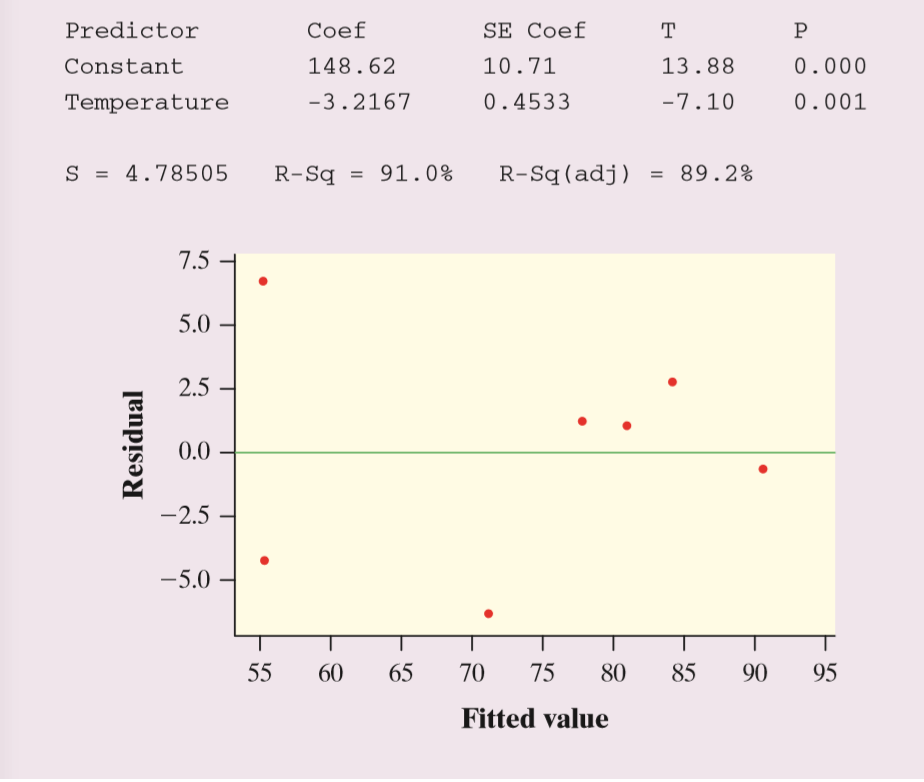
\includegraphics[scale=0.8]{figure0206}
    \end{figure}     
    
 \item What was the activity level rating for the fish at a temperature of 20\si{\degreeCelsius}?
     \begin{multicols}{5}
     \begin{enumerate}[(a)]
         \item 87   \item 84   \item 81    \item 66    \item 3
     \end{enumerate}
     \end{multicols}
     \vspace{0.3cm}
     
 \item Which of the following gives a correct interpretation of s in the above setting?
     \begin{enumerate}[(a)]
         \item For every 1\si{\degreeCelsius} increase in temperature, fish activity is predicted to increase by 4.785 units.
         \item The typical distance of the temperature readings from their mean is about 4.785\si{\degreeCelsius}.
         \item The typical distance of the activity level ratings from the least-squares line is about 4.785 units.
         \item The typical distance of the activity level readings from their mean is about 4.785.
         \item At a temperature of 0\si{\degreeCelsius}, this model predicts an activity level of 4.785.
     \end{enumerate}
     \vspace{0.3cm}
     
 \item Which of the following statements is not true of the correlation r between the lengths in inches and weights in pounds of a sample of brook trout?
 
     \begin{enumerate}[(a)]
         \item $r$ must take a value between $−1$ and 1.
         \item $r$ is measured in inches.
         \item If longer trout tend to also be heavier, then $r > 0$.
         \item $r$ would not change if we measured the lengths of the trout in centimeters instead of inches.
         \item $r$ would not change if we measured the weights of the trout in kilograms instead of pounds
     \end{enumerate}
     
 \item  When we standardize the values of a variable, the distribution of standardized values has mean 0 and standard  deviation 1. Suppose we measure two variables X and Y on each of several subjects. We standardize both variables and then compute the least-squares regression line. Suppose the slope of the least-squares regression line is $-0.44$. We may conclude that
        \begin{enumerate}[(a)]
            \item the intercept will also be $-0.44$.
            \item the intercept will be 1.0.
            \item the correlation will be 1/$-0.44$.
            \item the correlation will be 1.0.
            \item the correlation will also be $-0.44$.
        \end{enumerate}
        \vspace{0.3cm}
        
    \item There is a linear relationship between the number of chirps made by the striped ground cricket and the air temperature. A least-squares fit of some data collected by a biologist gives the model $\hat{y} =25.2+3.3\,x$, 
 where x is the number of chirps per minute and $\hat{y}$ is the estimated temperature in degrees Fahrenheit. What is the predicted increase in temperature for an increase of 5 chirps per minute?
        \begin{multicols}{5}
        \begin{enumerate}[(a)]
            \item 3.3 \si{\degree\farad}
            \item 16.5 \si{\degree\farad}
            \item 25.2 \si{\degree\farad}
            \item 28.5 \si{\degree\farad}
            \item 41.7 \si{\degree\farad}
        \end{enumerate}
        \end{multicols}
        \vspace{0.3cm}
        
    \item A data set included the number of people per  television set and the number of people per physician for 40 countries. The Fathom screen shot below displays a scatterplot of the data with the least-squares regression line added. In Ethiopia, there were 503 people per TV and 36,660 people per doctor. What effect would removing this point have on the regression line?
        \begin{figure}[H]
            \centering
            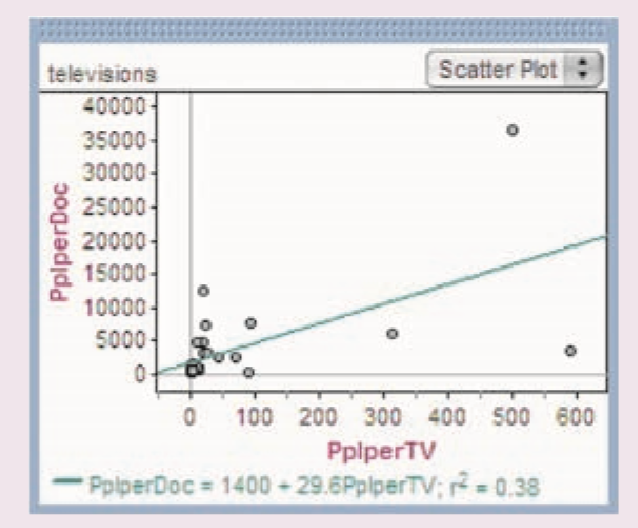
\includegraphics[scale=0.6]{figure0207}
        \end{figure}
    
        \begin{enumerate}[(a)]
            \item Slope would increase; y intercept would increase.
            \item Slope would increase; y intercept would decrease.
            \item Slope would decrease; y intercept would increase.
            \item Slope would decrease; y intercept would decrease.
            \item Slope and y intercept would stay the same
        \end{enumerate}
        \vspace{0.3cm}
        
    \item Suppose a study finds that the correlation coefficient relating family income to SAT scores is $r = +1$. Which of the following are proper conclusions?
         \begin{enumerate}[\Roman*. , start = 1]
             \item Poverty causes low SAT scores.
             \item Wealth causes high SAT scores.
             \item There is a very strong association between family income and SAT scores.
         \end{enumerate}
        
        \begin{multicols}{3}
        \begin{enumerate}[(a)]
            \item I only
            \item II only
            \item III only
            \item I and II
            \item I, II and III
        \end{enumerate}
        \end{multicols}
        \vspace{0.3cm}
        
    \item Consider the following three scatterplots:
        \begin{figure}[H]
            \centering
            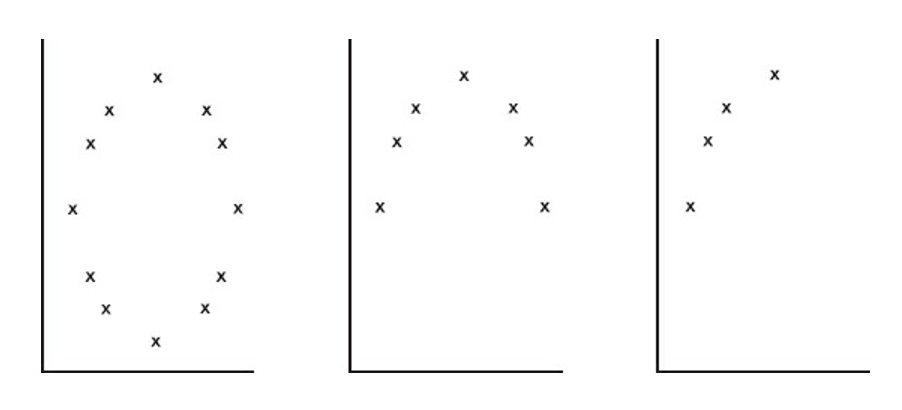
\includegraphics[scale=0.6]{figure0208}
        \end{figure}
        
        \begin{enumerate}[(a)]
            \item None are 0.
            \item One is 0, one is negative, and one is positive.
            \item One is 0, and both of the others are positive.
            \item Two are 0, and the other is 1.
            \item Two are 0, and the other is close to 1.
        \end{enumerate}
   \end{enumerate}
        \newpage    

    
    

\textbf{Free Response}

    \begin{enumerate}
        \item Using data from the 2010 census, a random sample of 348 U.S. residents aged 18 and older was selected. Among the variables recorded were gender (male or female), housing status (rent or own), and marital status (married or not married). 
        
        The two-way table below summarizes the relationship between gender and housing status.
        
        \begin{table}[H]
            \centering
            \begin{tabular}{cccc}
            \hline
            &\textbf{Male}&\textbf{Female}&\textbf{Total}\\
            Own&132&122&$\mathbf{254}$\\
            Rent&50&44&$\mathbf{94}$\\
            \textbf{Total}&$\mathbf{182}$&$\mathbf{166}$&$\mathbf{348}$\\
            \hline          
            \end{tabular}
        \end{table}
    
      \begin{enumerate}
          \item What percent of males in the sample own their home?
          \item Make a graph to compare the distribution of housing status for males and females. 
          \item Using your graph from part (b), describe the relationship between gender and housing status.
          \item The following two-way table below summarizes the relationship between marital status and housing status.
          
            \begin{table}[H]
            \centering
            \begin{tabular}{cccc}
            \hline
            &\textbf{Married}&\textbf{Not married}&\textbf{Total}\\
            Own&172&82&$\mathbf{254}$\\
            Rent&40&5554&$\mathbf{94}$\\
            \textbf{Total}&$\mathbf{212}$&$\mathbf{136}$&$\mathbf{348}$\\
            \hline          
            \end{tabular}
        \end{table}
          For the members of the sample, is the relationship between marital status and housing status stronger or weaker than the relationship between gender and housing status that you described in part (c)? Justify your choice using the data provided in the two-way tables. 
      \end{enumerate}  
      \newpage    
  
  \item \textbf{2007FR6}

A study was designed to explore subjects’ ability to judge the distance between two objects placed in a dimly lit room. The researcher suspected that the subjects would generally overestimate the distance between the objects in the room and that this overestimation would increase the farther apart the objects were.

The two objects were placed at random locations in the room before a subject estimated the distance (in feet) between those two objects. After each subject estimated the distance, the locations of the objects were rerandomized before the next subject viewed the room.

After data were collected for 40 subjects, two linear models were fit in an attempt to describe the relationship between the subjects’ perceived distances $(y)$ and the actual distance, in feet, between the two objects.

\begin{center}
{Model 1: $\hat{y} =0.238+1.080 \times$(actual distance)}
\end{center}

The standard errors of the estimated coefficients for Model 1 are 0.260 and 0.118, respectively.

\begin{center}
Model 2: $\hat{y}=1.102\times$(actual distance)
\end{center}

The standard error of the estimated coefficient for Model 2 is 0.393.
  
  \begin{enumerate}[(a), start = 1]
  \item  Provide an interpretation in context for the estimated slope in Model 1.
  \item Explain why the researcher might prefer Model 2 to Model 1 in this context.
  \item Using Model 2, test the researcher’s hypothesis that in dim light participants overestimate the distance, with the overestimate increasing as the actual distance increases. (Assume appropriate conditions for inference are met.)
  \end{enumerate}
  
The researchers also wanted to explore whether the performance on this task differed between subjects who wear contact lenses and subjects who do not wear contact lenses. A new variable was created to indicate whether or not a subject wears contact lenses. The data for this variable were coded numerically (1 = contact wearer, 0 = noncontact wearer), and this new variable, named “contact,” was included in the following model.\\

\begin{center}
Model 3:$\hat{y}=1.0\times$(actual distance)+$0.12\times$(contact)$\times$(actual distance) 
\end{center}
The standard errors of the estimated coefficients for Model 3 are 0.357 and 0.032, respectively.
  
   \begin{enumerate}[(a), resume]
   \item Using Model 3, sketch the estimated regression model for contact wearers and the estimated regression model for noncontact wearers on the grid below.\\
   \begin{center}
   {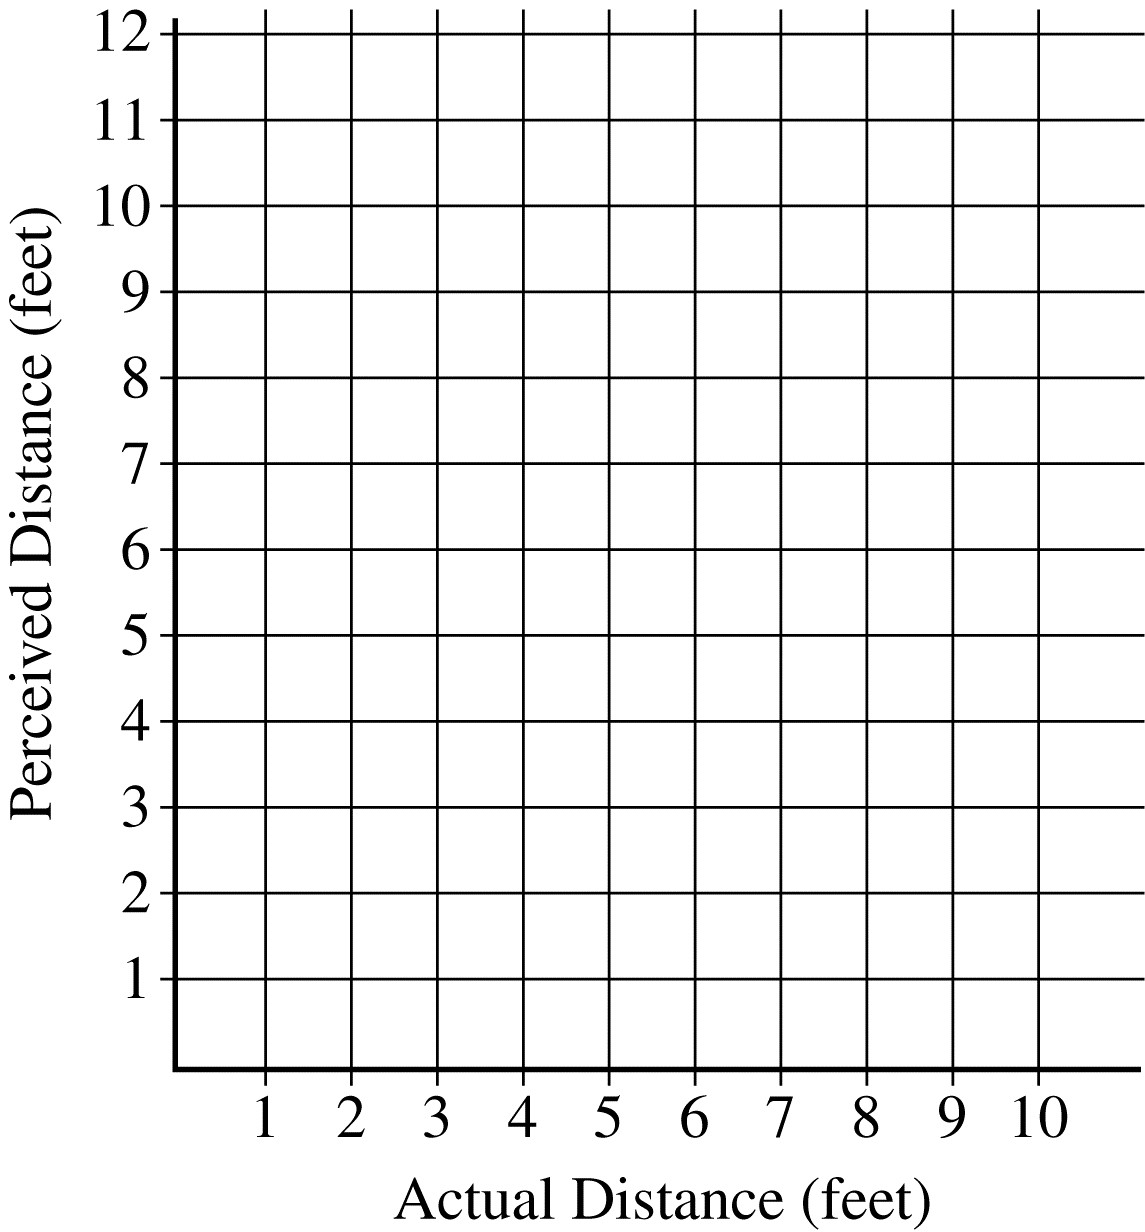
\includegraphics[scale=0.15]{2007FR6-1.JPG}}
   \end{center}
    \item   In the context of this study, provide an interpretation of the estimated coefficients for \mbox{Model 3}.
   \end{enumerate}
   \newpage
   
 \item \textbf{2007FRB4}\\
   Each of 25 adult women was asked to provide her own height (y), in inches, and the height (x), in inches, of her father. The scatterplot below displays the results. Only 22 of the 25 pairs are distinguishable because some of the (x,y) pairs were the same. The equation of the least squares regression line is $\hat{y}=35.1+0.427x$
   \begin{center}
   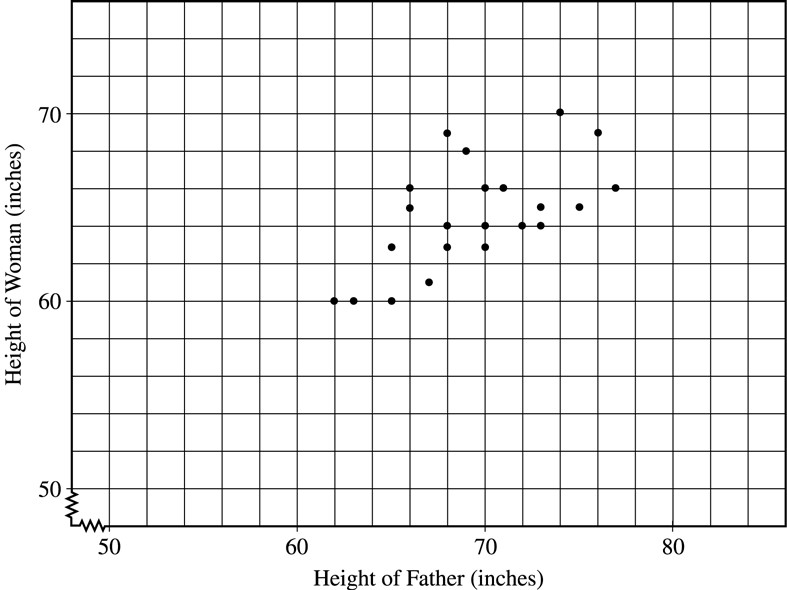
\includegraphics[scale=0.4]{2007FRB4-1.JPG}
   \end{center}
   
  \begin{enumerate}[(a), start =1]
   \item  Draw the least squares regression line on the scatterplot above.
   \item One father’s height was x = 67 inches and his daughter’s height was y = 61 inches. Circle the point on the scatterplot above that represents this pair and draw the segment on the scatterplot that corresponds to the residual for it. Give a numerical value for the residual.
   \item Suppose the point x = 84, y = 71 is added to the data set. Would the slope of the least squares regression line increase, decrease, or remain about the same? Explain. (Note: No calculations are necessary to answer this question.)\\
   Would the correlation increase, decrease, or remain about the same? Explain. (Note: No calculations are necessary to answer this question.)
  \end{enumerate}
  \newpage
  
  
\item \textbf{2014FR6}\\
Jamal is researching the characteristics of a car that might be useful in predicting the fuel consumption rate (FCR); that is, the number of gallons of gasoline that the car requires to travel 100 miles under conditions of typical city driving. The length of a car is one explanatory variable that can be used to predict FCR. Graph I is a scatterplot showing the lengths of 66 cars plotted with the corresponding FCR. One point on the graph is labeled A.
  
    \begin{center}
      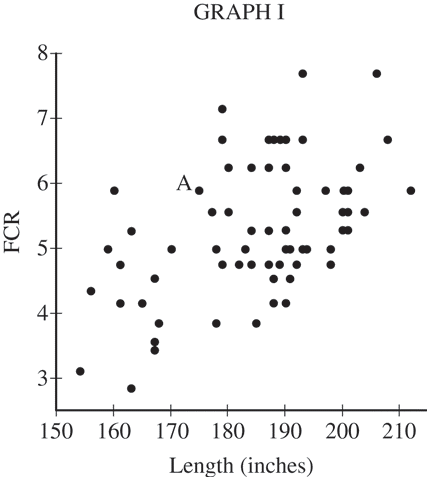
\includegraphics[scale=0.5]{2014FR6-1.PNG}
    \end{center}
    
Jamal examined the scatterplot and determined that a linear model would be a reasonable way to express the relationship between FCR and length. A computer output from a linear regression is shown below.

   \begin{center}
       \begin{tabular}{ll}
       \multicolumn{2}{l}{Linear Fit}\\
       \multicolumn{2}{l}{FCR$=-1.595789+0.0372614\times$Length}\\
       &\\
       \multicolumn{2}{l}{Summary of Fit}\\
       R-square & 0.250401\\
       Root Mean Square Error &	0.902382\\
       Observations	& 66\\ 
       \end{tabular}
   \end{center}
  
     \begin{enumerate}[(a), start = 1]
      \item  The point on the graph labeled A represents one car of length 175 inches and an FCR of 5.88. Calculate and interpret the residual for the car relative to the least squares regression line.\\
    
    \item  Jamal knows that it is possible to predict a response variable using more than one explanatory variable. He wants to see if he can improve the original model of predicting FCR from length by including a second explanatory variable in addition to length. He is considering including engine size, in liters, or wheel base (the length between axles), in inches. Graph II is a scatterplot showing the engine size of the 66 cars plotted with the corresponding residuals from the regression of FCR on length. Graph III is a scatterplot showing the wheel base of the 66 cars plotted with the corresponding residuals from the regression of FCR on length.
      \begin{center}
        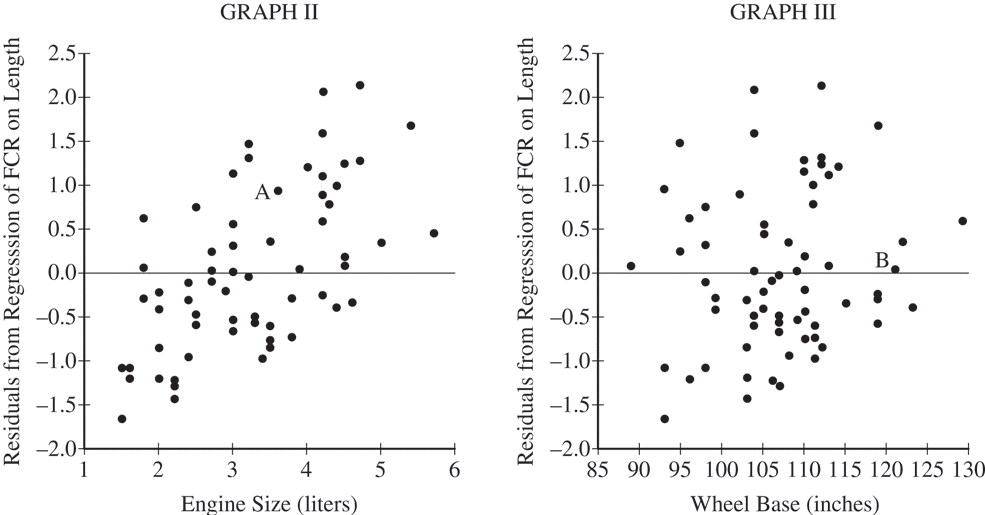
\includegraphics[scale=0.4]{2014FR6-2.PNG}
      \end{center}
      In graph II, the point labeled A corresponds to the same car whose point was labeled A in graph I. The measurements for the car represented by point A are given below.
      
        \begin{center}
          \begin{tabular}{*{4}{|c}|}
          \hline
          FCR&Length(inches)&Engine Size (liters)&Wheel Base (inches)\\
          \hline
          5.88&175&3.6&93\\
          \hline
          \end{tabular}
        \end{center}
        
          \begin{enumerate}[(\roman*), start = 1]
           \item  Circle the point on graph III that corresponds to the car represented by point A on graphs I and II.
           \item There is a point on graph III labeled B. It is very close to the horizontal line at 0. What does that indicate about the FCR of the car represented by point B?
          \end{enumerate}
     \vspace{0.5cm}
          
      \item Write a few sentences to compare the association between the variables in graph II with the association between the variables in graph III.\\
      
      \item  Jamal wants to predict FCR using length and one of the other variables, engine size or wheel base. Based on your response to part (c), which variable, engine size or wheel base, should Jamal use in addition to length if he wants to improve the prediction? Explain why you chose that variable.
     \end{enumerate}
     \newpage
     
 \item \textbf{2015FR5}\\
  A student measured the heights and the arm spans, rounded to the nearest inch, of each person in a random sample of 12 seniors at a high school. A scatterplot of arm span versus height for the 12 seniors is shown.
  \begin{center}
    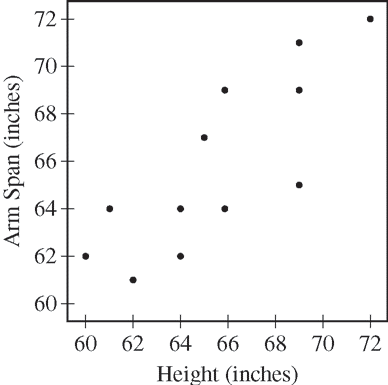
\includegraphics[scale=0.5]{2015FR5-1.PNG}
  \end{center}
    \begin{enumerate}[(a), start = 1]
     \item   Based on the scatterplot, describe the relationship between arm span and height for the sample of 12 seniors. Let x represent height, in inches, and let y represent arm span, in inches. Two scatterplots of the same data are shown below. Graph 1 shows the data with the least squares regression line
     $$\hat{y}=11.74+0.8247x$$
     And graph 2 shows the data with the line $y=x$ .
     \begin{center}
    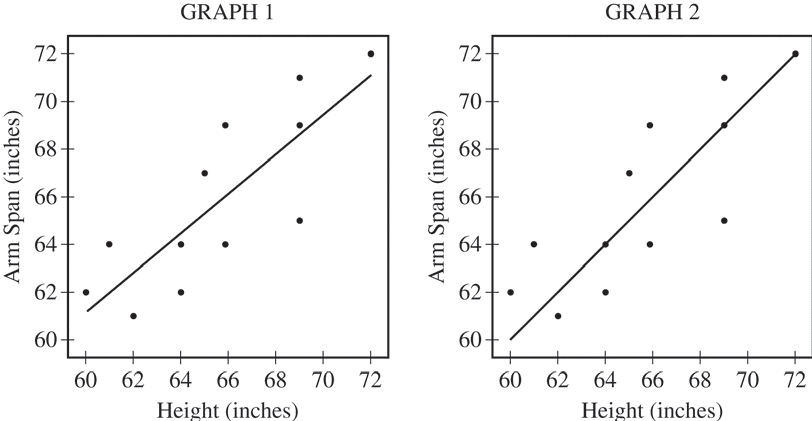
\includegraphics[scale=0.5]{2015FR5-2.PNG}
  \end{center}
   \item  The criteria described in the table below can be used to classify people into one of three body shape categories: square, tall rectangle, or short rectangle.
   
    \begin{table}[H]
    \hspace{-3cm}
      \begin{tabular}{|c|c|c|}
      \hline
      Square&Tall Rectangle&Short Rectangle\\
      \hline
      Arm span is equal to height.&Arm span is less than height.&Arm span is greater than height.\\
      \hline
      \end{tabular}
    \end{table}
  \vspace{0.5cm}
    \begin{enumerate}[(\roman*), start = 1]
     \item  For which graph, 1 or 2, is the line helpful in classifying a student’s body shape as square, tall rectangle, or short rectangle? Explain.
     \item Complete the table of classifications for the 12 seniors.
 \vspace{0.5cm}    
       \begin{center}
         \begin{tabular}{|c|c|c|c|}
         \hline
           Classification&Square&Tall Rectangle&Short Rectangle\\
           \hline
           Frequency&&&\\
           \hline
         \end{tabular}
       \end{center}
    
    \end{enumerate}
     \item   Using the best model for prediction, calculate the predicted arm span for a senior with height 61 inches.
    
    \end{enumerate}
    
    \end{enumerate}







\end{document}